\documentclass[tikz,convert={outfile=\jobname.svg}]{standalone}
\usetikzlibrary{calc,patterns,snakes}
% \usetikzlibrary{...}% tikz package already loaded by 'tikz' option
\begin{document}
  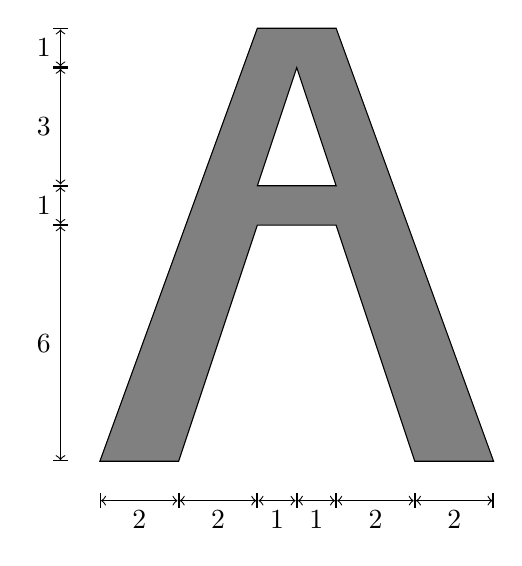
\begin{tikzpicture}[scale=0.5]
    \draw[fill=gray] (0, 0) -- (2, 0) -- (4, 6) -- (6, 6) -- (8, 0) -- (10, 0) -- (6, 11) -- (4, 11) -- cycle;
    \draw[fill=white] (4, 7) -- (6, 7) -- (5, 10) -- cycle;
    \foreach \x in {0, 1} {
      \draw[|<->|] (0+2*\x, -1) -- (2+2*\x, -1) node[midway, below] {$2$};
      }
    \foreach \x in {3, 4} {
      \draw[|<->|] (0+2*\x, -1) -- (2+2*\x, -1) node[midway, below] {$2$};
      }
    \draw[|<->|] (4, -1) -- (5, -1) node[midway, below] {$1$};
    \draw[|<->|] (5, -1) -- (6, -1) node[midway, below] {$1$};
    \draw[|<->|] (-1, 0) -- (-1, 6) node[midway, left]{$6$};
    \draw[|<->|] (-1, 6) -- (-1, 7) node[midway, left]{$1$};
    \draw[|<->|] (-1, 7) -- (-1, 10) node[midway, left]{$3$};
    \draw[|<->|] (-1, 10) -- (-1, 11) node[midway, left]{$1$};
  \end{tikzpicture}
\end{document}